\documentclass[11pt,a4paper]{report}
\usepackage[textwidth=37em,vmargin=30mm]{geometry}
\usepackage{calc,xunicode,amsmath,amssymb,paralist,enumitem,tabu,booktabs,datetime2,xeCJK,xeCJKfntef,listings}
\usepackage{tocloft,fancyhdr,tcolorbox,xcolor,graphicx,eso-pic,xltxtra,xelatexemoji}

\newcommand{\envyear}[0]{2025}
\newcommand{\envdatestr}[0]{2025-07-29}
\newcommand{\envfinaldir}[0]{webdb/2025/20250729/final}

\usepackage[hidelinks]{hyperref}
\hypersetup{
    colorlinks=false,
    pdfpagemode=FullScreen,
    pdftitle={Web Digest - \envdatestr}
}

\setlength{\cftbeforechapskip}{10pt}
\renewcommand{\cftchapfont}{\rmfamily\bfseries\large\raggedright}
\setlength{\cftbeforesecskip}{2pt}
\renewcommand{\cftsecfont}{\sffamily\small\raggedright}

\setdefaultleftmargin{2em}{2em}{1em}{1em}{1em}{1em}

\usepackage{xeCJK,xeCJKfntef}
\xeCJKsetup{PunctStyle=plain,RubberPunctSkip=false,CJKglue=\strut\hskip 0pt plus 0.1em minus 0.05em,CJKecglue=\strut\hskip 0.22em plus 0.2em}
\XeTeXlinebreaklocale "zh"
\XeTeXlinebreakskip = 0pt


\setmainfont{Brygada 1918}
\setromanfont{Brygada 1918}
\setsansfont{IBM Plex Sans}
\setmonofont{JetBrains Mono NL}
\setCJKmainfont{Noto Serif CJK SC}
\setCJKromanfont{Noto Serif CJK SC}
\setCJKsansfont{Noto Sans CJK SC}
\setCJKmonofont{Noto Sans CJK SC}

\setlength{\parindent}{0pt}
\setlength{\parskip}{8pt}
\linespread{1.15}

\lstset{
	basicstyle=\ttfamily\footnotesize,
	numbersep=5pt,
	backgroundcolor=\color{black!5},
	showspaces=false,
	showstringspaces=false,
	showtabs=false,
	tabsize=2,
	captionpos=b,
	breaklines=true,
	breakatwhitespace=true,
	breakautoindent=true,
	linewidth=\textwidth
}






\newcommand{\coverpic}[2]{
    % argv: itemurl, authorname
    Cover photo by #2~~(\href{#1}{#1})
}
\newcommand{\makeheader}[0]{
    \begin{titlepage}
        % \newgeometry{hmargin=15mm,tmargin=21mm,bmargin=12mm}
        \begin{center}
            
            \rmfamily\scshape
            \fontspec{BaskervilleF}
            \fontspec{Old Standard}
            \fontsize{59pt}{70pt}\selectfont
            WEB\hfill DIGEST
            
            \vfill
            % \vskip 30pt
            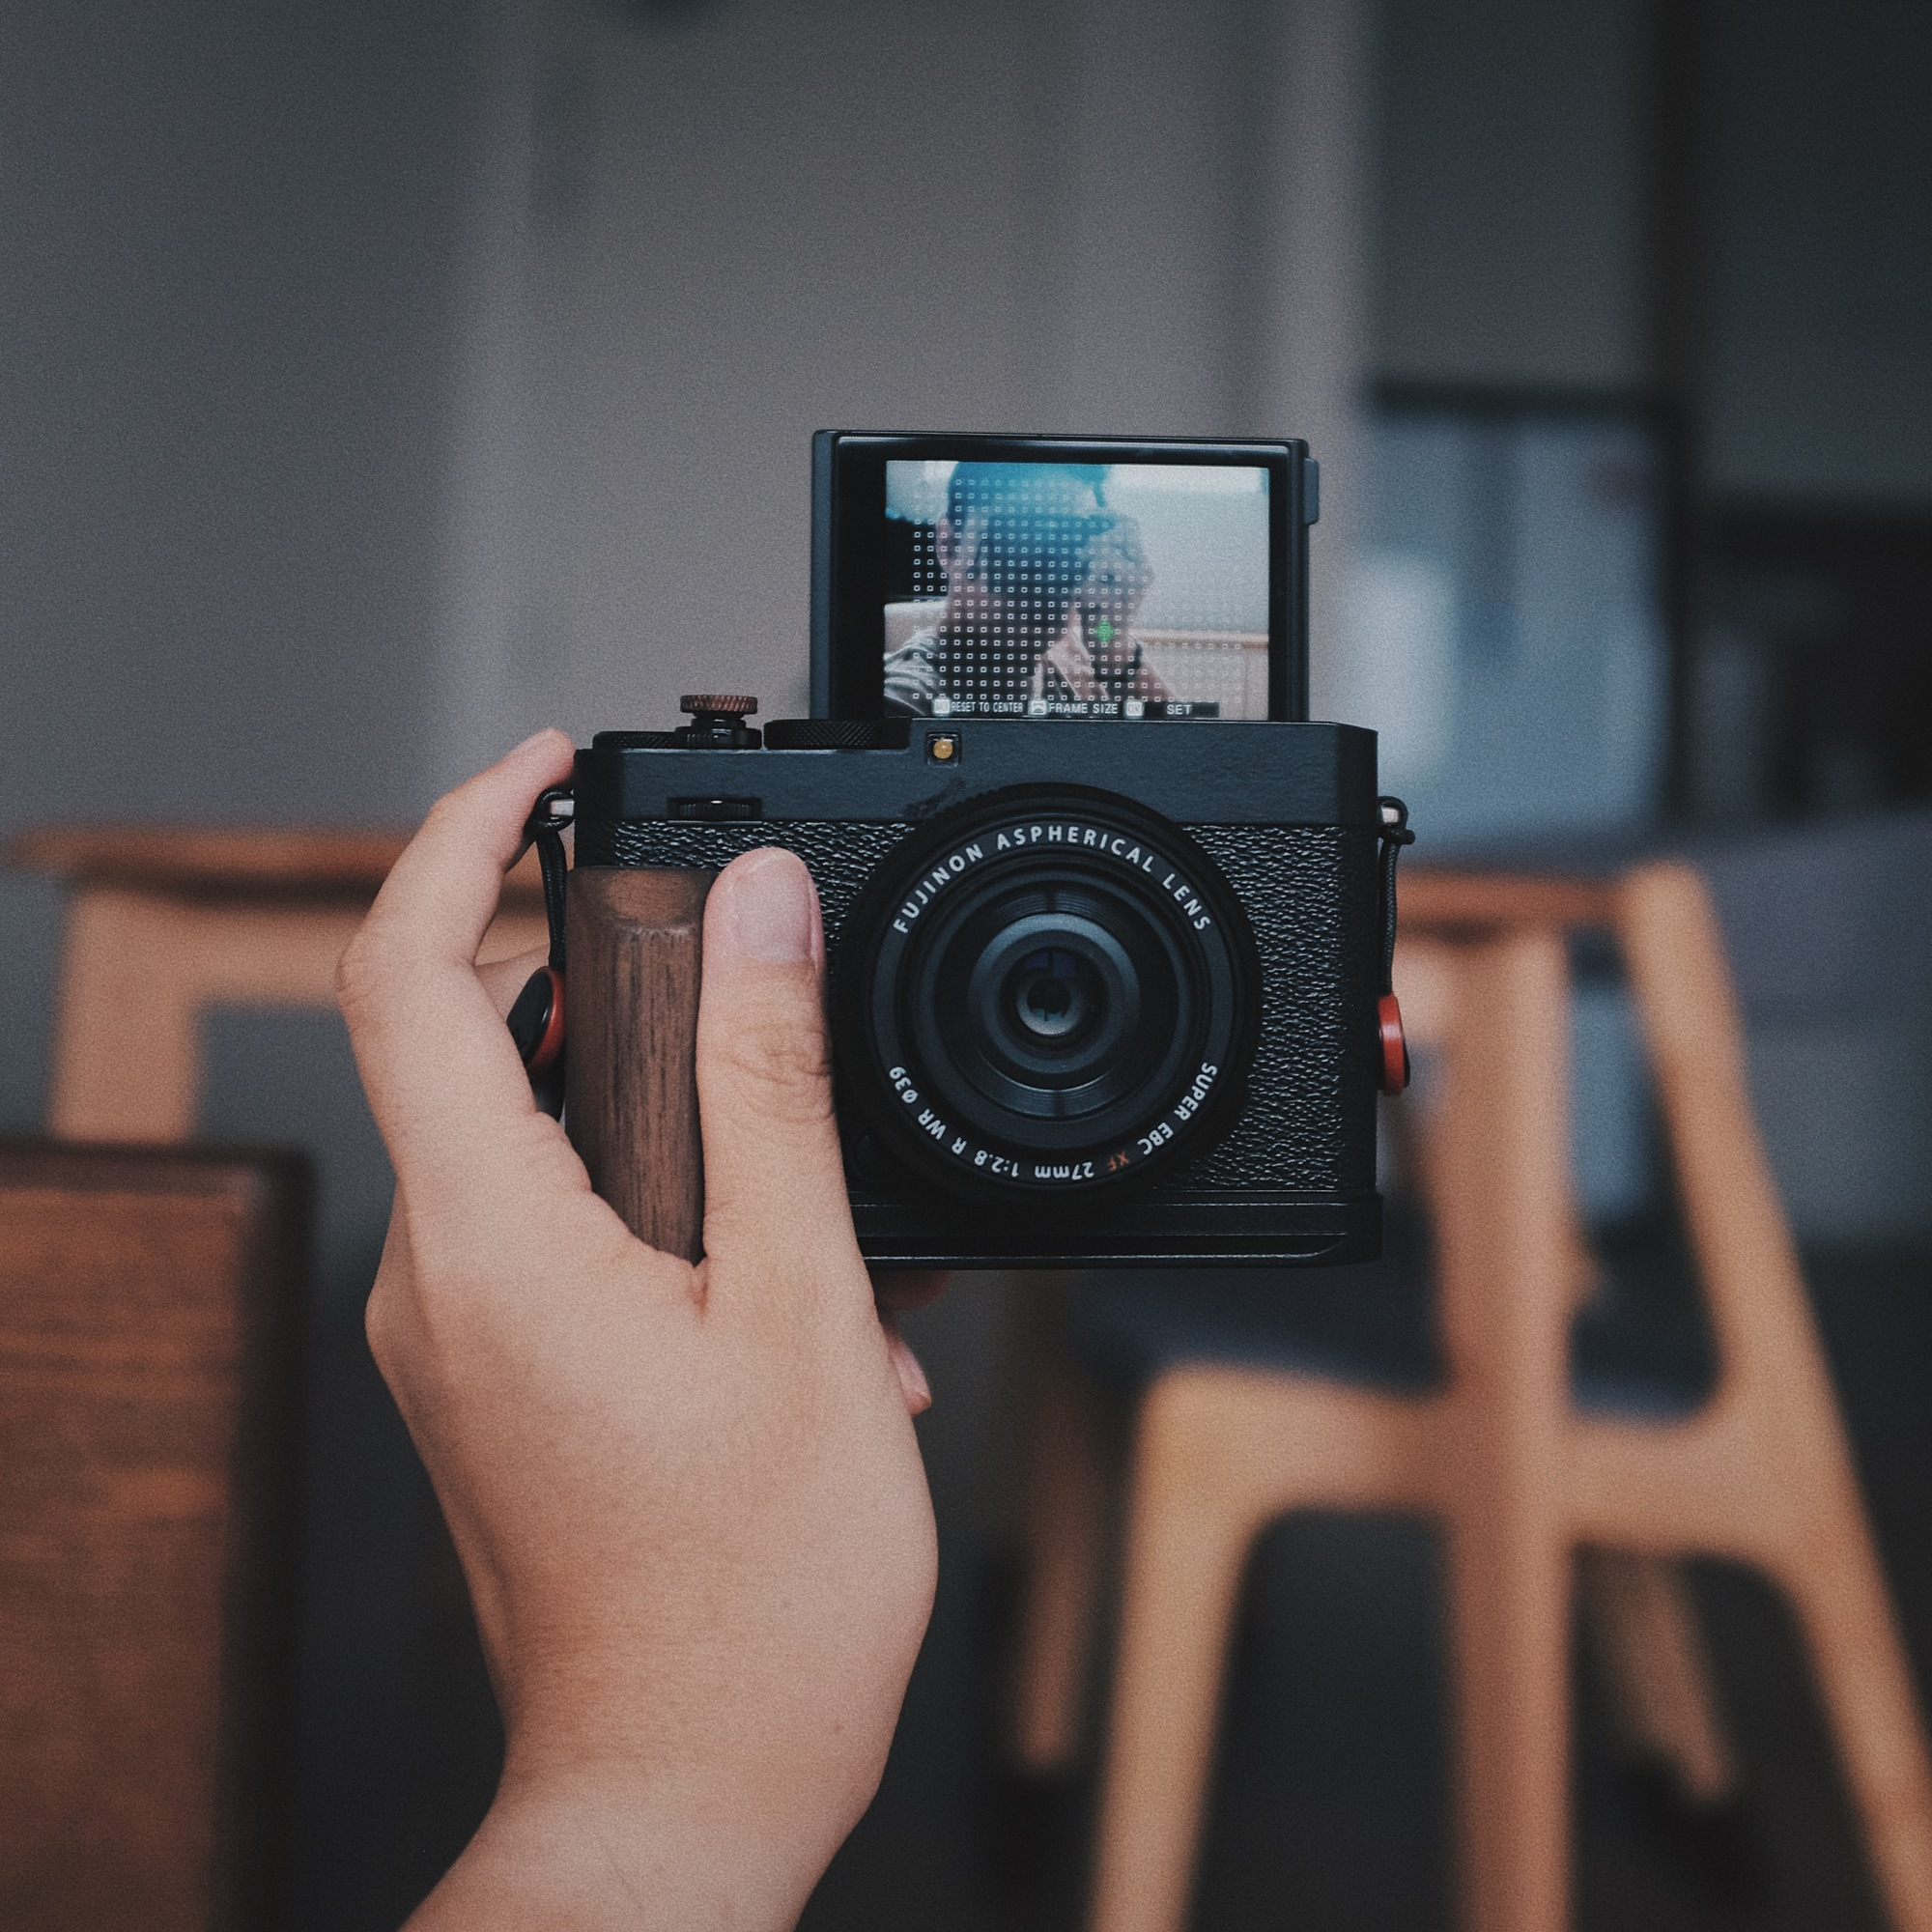
\includegraphics[width=\linewidth]{\envfinaldir/coverpic-prod.jpg}\par
            % \vskip 30pt
            \vfill

            \normalsize\rmfamily\scshape
            \copyright{} The Web Digest Project \hfill\large \envdatestr
        \end{center}
    \end{titlepage}
    % \restoregeometry
}
\newcommand{\simplehref}[1]{%
    \textcolor{blue!80!green}{\href{#1}{#1}}%
}
\renewcommand{\contentsname}{\center\Huge\sffamily\bfseries Contents\par\vskip 20pt}
\newcounter{ipartcounter}
\setcounter{ipartcounter}{0}
\newcommand{\ipart}[1]{
    % \vskip 20pt
    \clearpage
    \stepcounter{ipartcounter}
    \phantomsection
    \addcontentsline{toc}{chapter}{#1}
    % \begin{center}
    %     \Huge
    %     \sffamily\bfseries
    %     #1
    % \end{center}
    % \vskip 20pt plus 7pt
}
\newcounter{ichaptercounter}
\setcounter{ichaptercounter}{0}
\newcommand{\ichapter}[1]{
    % \vskip 20pt
    \clearpage
    \stepcounter{ichaptercounter}
    \phantomsection
    \addcontentsline{toc}{section}{\numberline{\arabic{ichaptercounter}}#1}
    \begin{center}
        \Huge
        \sffamily\bfseries
        #1
    \end{center}
    \vskip 20pt plus 7pt
}
\newcommand{\entrytitlefont}[1]{\subsection*{\raggedright\Large\sffamily\bfseries#1}}
\newcommand{\entryitemGeneric}[2]{
    % argv: title, url
    \parbox{\linewidth}{
        \entrytitlefont{#1}\par\vskip 5pt
        \footnotesize\ttfamily\mdseries
        \simplehref{#2}
    }\vskip 11pt plus 11pt minus 1pt
}
\newcommand{\entryitemGithub}[3]{
    % argv: title, url, desc
    \parbox{\linewidth}{
        \entrytitlefont{#1}\par\vskip 5pt
        \footnotesize\ttfamily\mdseries
        \simplehref{#2}\par\vskip 5pt
        \small\rmfamily\mdseries#3
    }\vskip 11pt plus 11pt minus 1pt
}
\newcommand{\entryitemAp}[3]{
    % argv: title, url, desc
    \parbox{\linewidth}{
        \entrytitlefont{#1}\par\vskip 5pt
        \footnotesize\ttfamily\mdseries
        \simplehref{#2}\par\vskip 5pt
        \small\rmfamily\mdseries#3
    }\vskip 11pt plus 11pt minus 1pt
}
\newcommand{\entryitemHackernews}[3]{
    % argv: title, hnurl, rawurl
    % \parbox{\linewidth}{
    %     \entrytitlefont{#1}\par\vskip 5pt
    %     \footnotesize\ttfamily\mdseries
    %     \simplehref{#3}\par
    %     \textcolor{black!50}{\href{#2}{#2}}
    % }\vskip 11pt plus 11pt minus 1pt
    \begin{minipage}{\linewidth}
            \entrytitlefont{#1}\par\vskip 5pt
            \footnotesize\ttfamily\mdseries
            \simplehref{#3}\par
            \textcolor{black!50}{\href{#2}{#2}}
    \end{minipage}\par\vskip 11pt plus 11pt minus 1pt
}







\begin{document}

\makeheader

\tableofcontents\clearpage




\ipart{Developers}
\ichapter{Hacker News}
\entryitemTwoLinks{Show HN: Use Their ID – Use Your Local UK MP's ID for the Online Safety Act}{https://news.ycombinator.com/item?id=44716106}{https://use-their-id.com/}

\entryitemTwoLinks{Sign in with Google in Chrome}{https://news.ycombinator.com/item?id=44715166}{https://underpassapp.com/news/2025/7/5.html}

\entryitemTwoLinks{I designed my own fast game streaming video codec – PyroWave}{https://news.ycombinator.com/item?id=44714914}{https://themaister.net/blog/2025/06/16/i-designed-my-own-ridiculously-fast-game-streaming-video-codec-pyrowave/}

\entryitemTwoLinks{Different Clocks}{https://news.ycombinator.com/item?id=44714223}{https://ianto-cannon.github.io/clock.html}

\entryitemTwoLinks{`I witnessed war crimes' in Gaza – former worker at GHF aid site [video]}{https://news.ycombinator.com/item?id=44714221}{https://www.bbc.com/news/videos/cy8k8045nx9o}

\entryitemTwoLinks{Claude Code weekly rate limits}{https://news.ycombinator.com/item?id=44713757}{https://news.ycombinator.com/item?id=44713757}

\entryitemTwoLinks{Visa and Mastercard are getting overwhelmed by gamer fury over censorship}{https://news.ycombinator.com/item?id=44713414}{https://www.polygon.com/news/616835/visa-mastercard-steam-itchio-campaign-adult-games}

\entryitemTwoLinks{I saved a PNG image to a bird}{https://news.ycombinator.com/item?id=44712311}{https://www.youtube.com/watch?v=hCQCP-5g5bo}

\entryitemTwoLinks{More women than expected are genetically men (2016)}{https://news.ycombinator.com/item?id=44711836}{https://novonordiskfonden.dk/en/news/more-women-than-expected-are-genetically-men/}

\entryitemTwoLinks{Simplify, then add delightness: On designing for children}{https://news.ycombinator.com/item?id=44711745}{https://shaneosullivan.wordpress.com/2025/07/28/on-designing-for-children/}

\entryitemTwoLinks{FDA has approved Yeztugo, a drug that provides protection against HIV infection}{https://news.ycombinator.com/item?id=44711612}{https://newatlas.com/infectious-diseases/hiv-prevention-fda-lenacapavir/}

\entryitemTwoLinks{Copyparty – Turn almost any device into a file server}{https://news.ycombinator.com/item?id=44711519}{https://github.com/9001/copyparty}

\entryitemTwoLinks{Tao on ``blue team'' vs. ``red team'' LLMs}{https://news.ycombinator.com/item?id=44711306}{https://mathstodon.xyz/@tao/114915604830689046}

\entryitemTwoLinks{GLM-4.5: Reasoning, Coding, and Agentic Abililties}{https://news.ycombinator.com/item?id=44711106}{https://z.ai/blog/glm-4.5}

\entryitemTwoLinks{Show HN: I made a tool to generate photomosaics with your pictures}{https://news.ycombinator.com/item?id=44709727}{https://pictiler.com}

\entryitemTwoLinks{Debian switches to 64-bit time for everything}{https://news.ycombinator.com/item?id=44709408}{https://www.theregister.com/2025/07/25/y2k38\_bug\_debian/}

\entryitemTwoLinks{How to make websites that will require lots of your time and energy}{https://news.ycombinator.com/item?id=44708270}{https://blog.jim-nielsen.com/2025/how-to-make-websites-that-require-lots-of-time-and-energy/}

\entryitemTwoLinks{What would an efficient and trustworthy meeting culture look like?}{https://news.ycombinator.com/item?id=44708173}{https://abitmighty.com/posts/the-ultimate-meeting-culture}

\entryitemTwoLinks{LLM Embeddings Explained: A Visual and Intuitive Guide}{https://news.ycombinator.com/item?id=44708028}{https://huggingface.co/spaces/hesamation/primer-llm-embedding}

\entryitemTwoLinks{SIMD within a register: How I doubled hash table lookup performance}{https://news.ycombinator.com/item?id=44707546}{https://maltsev.space/blog/012-simd-within-a-register-how-i-doubled-hash-table-lookup-performance}


\ipart{Developers~~~~(zh-Hans)}
\ichapter{V2EX}
\entryitemGeneric{\hskip 0pt{}[问与答] 北京今天有多少居家办公的?}{https://www.v2ex.com/t/1148369}

\entryitemGeneric{\hskip 0pt{}[酷工作] (远程,可兼职) GenAI 创业团队招前端开发,产品已上线}{https://www.v2ex.com/t/1148368}

\entryitemGeneric{\hskip 0pt{}[游戏] 唉,想玩 16 年的守望先锋,想玩 17 年的黎明杀鸡、彩虹六号}{https://www.v2ex.com/t/1148367}

\entryitemGeneric{\hskip 0pt{}[问与答] 或许可以用育儿补贴数估算新生儿数量?}{https://www.v2ex.com/t/1148366}

\entryitemGeneric{\hskip 0pt{}[iOS] 坚持 iOS 17.6.1 与 iOS 18.3.1,五年不变}{https://www.v2ex.com/t/1148365}

\entryitemGeneric{\hskip 0pt{}[宽带症候群] TCP-over-TCP 的性能陷阱,大家有实际遇到过吗?}{https://www.v2ex.com/t/1148364}

\entryitemGeneric{\hskip 0pt{}[加密货币] 国内注册的币安,现在居住在澳洲提示 IP 错误}{https://www.v2ex.com/t/1148363}

\entryitemGeneric{\hskip 0pt{}[Solana] V2EX 的 Solana 介绍页面现在会显示 V2EX 的 Solana 场景的一些实时数据}{https://www.v2ex.com/t/1148362}

\entryitemGeneric{\hskip 0pt{}[酷工作] [上海/广州/北京] 训练/推理平台开发工程师}{https://www.v2ex.com/t/1148360}

\entryitemGeneric{\hskip 0pt{}[Solana] 能不能上所啊 舞起来}{https://www.v2ex.com/t/1148359}

\entryitemGeneric{\hskip 0pt{}[程序员] 有没有开源类似淘宝的简易多商户买卖系统}{https://www.v2ex.com/t/1148358}

\entryitemGeneric{\hskip 0pt{}[Apple] 苹果公司首次在中国关闭直营店}{https://www.v2ex.com/t/1148356}

\entryitemGeneric{\hskip 0pt{}[分享创造] 朋友是汉语老师,给小朋友取中文名太费脑子,我做了个 AI 工具帮她}{https://www.v2ex.com/t/1148355}

\entryitemGeneric{\hskip 0pt{}[Android] 小米 13 澎湃 1.0.7,今天突然搜不到 wifi 了}{https://www.v2ex.com/t/1148353}

\entryitemGeneric{\hskip 0pt{}[剧集] 凡人修仙传,韩立离村远看亲人时,是否太绝情?}{https://www.v2ex.com/t/1148352}

\entryitemGeneric{\hskip 0pt{}[酷工作] ⼤模型算法研究⼯程师, Base 湾区,提供工作签证}{https://www.v2ex.com/t/1148348}

\entryitemGeneric{\hskip 0pt{}[酷工作] 北京-快手-内推鸿蒙开发工程师-欢迎对鸿蒙稳定性感兴趣的小伙伴投递}{https://www.v2ex.com/t/1148346}

\entryitemGeneric{\hskip 0pt{}[Solana] 请教一下 solana 或则 V2EX 代币怎么购买}{https://www.v2ex.com/t/1148345}

\entryitemGeneric{\hskip 0pt{}[分享创造] Docker 部署多节点 Looking Glass 面板 NetMirror}{https://www.v2ex.com/t/1148344}

\entryitemGeneric{\hskip 0pt{}[Android] 安卓的 root 信息应该去哪里查? pixel 的手机}{https://www.v2ex.com/t/1148342}

\entryitemGeneric{\hskip 0pt{}[推广] 跪求天翼云客户~~月底了~~~~}{https://www.v2ex.com/t/1148341}

\entryitemGeneric{\hskip 0pt{}[Apple] 新买的国行 iPhone 14 无法访问币安 binance.com, 但能访问 google/以太坊, why?}{https://www.v2ex.com/t/1148340}

\entryitemGeneric{\hskip 0pt{}[分享发现] [记录]-2025-07-28 一辆 Go Kart}{https://www.v2ex.com/t/1148339}

\entryitemGeneric{\hskip 0pt{}[写周报] 独立开发周记 128:爆单、爆肝、爆米花}{https://www.v2ex.com/t/1148337}

\entryitemGeneric{\hskip 0pt{}[问与答] 熊猫吃短信 1 的数据还更新不? app 五个月没更了}{https://www.v2ex.com/t/1148336}

\entryitemGeneric{\hskip 0pt{}[奇思妙想] 想法:阅读计时这样的软件或者功能,是伪需求吗?}{https://www.v2ex.com/t/1148335}

\entryitemGeneric{\hskip 0pt{}[互联网] 大家开发的 web app 是如何解决支付问题的?}{https://www.v2ex.com/t/1148332}

\entryitemGeneric{\hskip 0pt{}[宽带症候群] 安徽电信宽带一直有问题}{https://www.v2ex.com/t/1148331}

\entryitemGeneric{\hskip 0pt{}[酷工作] 上海杨浦区: Android 开发工程师, 2 个星期短期项目}{https://www.v2ex.com/t/1148330}

\entryitemGeneric{\hskip 0pt{}[程序员] Amazon Q 的大瓜, 自动清理所有 AWS 资源, 欣赏一下注入的提示词}{https://www.v2ex.com/t/1148329}

\entryitemGeneric{\hskip 0pt{}[深圳] 老婆孕期被辞退,有什么可以争取的}{https://www.v2ex.com/t/1148328}

\entryitemGeneric{\hskip 0pt{}[问与答] 公司想科学上网拉点 github、gitlab、aws 的代码有什么措施吗?}{https://www.v2ex.com/t/1148326}

\entryitemGeneric{\hskip 0pt{}[生活] 找房有感,刚需盘就是个大型韭菜盒子}{https://www.v2ex.com/t/1148325}

\entryitemGeneric{\hskip 0pt{}[生活] 你们是怎么买温度计的?电子的还是机械的?}{https://www.v2ex.com/t/1148324}

\entryitemGeneric{\hskip 0pt{}[生活] 有腰突的朋友吗}{https://www.v2ex.com/t/1148323}

\entryitemGeneric{\hskip 0pt{}[问与答] 哈罗奖励金是永久下架了吗}{https://www.v2ex.com/t/1148321}

\entryitemGeneric{\hskip 0pt{}[酷工作] 大厂直招薪资 60~ 100+}{https://www.v2ex.com/t/1148318}

\entryitemGeneric{\hskip 0pt{}[Solana] V2EX 在 Phantom 买和在交易所买差别大吗}{https://www.v2ex.com/t/1148317}

\entryitemGeneric{\hskip 0pt{}[问与答] 香港手机卡能做什么?}{https://www.v2ex.com/t/1148315}

\entryitemGeneric{\hskip 0pt{}[全球工单系统] 吐槽 Moji 辭書}{https://www.v2ex.com/t/1148313}

\entryitemGeneric{\hskip 0pt{}[问与答] 如何接入 Stripe?}{https://www.v2ex.com/t/1148312}

\entryitemGeneric{\hskip 0pt{}[宽带症候群] 求推荐支持 Https 协议的正向代理软件}{https://www.v2ex.com/t/1148310}

\entryitemGeneric{\hskip 0pt{}[深圳] 深圳 75 平人才房(套内小)求推荐性价比家电家私}{https://www.v2ex.com/t/1148309}

\entryitemGeneric{\hskip 0pt{}[问与答] 企微文档中的流程图如何复制或导出到外部 drawio 编辑?}{https://www.v2ex.com/t/1148307}

\entryitemGeneric{\hskip 0pt{}[VPS] 无套路 [抽奖送一个 VPS 使用权 1 个月] 限 1 人,今晚 8 点开}{https://www.v2ex.com/t/1148305}

\entryitemGeneric{\hskip 0pt{}[生活] 人心中的成见是大山,怎么说服父亲把老破小卖了?}{https://www.v2ex.com/t/1148304}

\entryitemGeneric{\hskip 0pt{}[酷工作] [广州][Android]海外社交产品团队招研发,项目已获千万级美元融资| 2025 Q3 发布| Q4 美国 IPO}{https://www.v2ex.com/t/1148303}

\entryitemGeneric{\hskip 0pt{}[程序员] 分布式锁是否能实现锁住一个 key 范围}{https://www.v2ex.com/t/1148302}

\entryitemGeneric{\hskip 0pt{}[生活] 各位是怎么除蟑螂的?有啥有效的方法么}{https://www.v2ex.com/t/1148301}

\entryitemGeneric{\hskip 0pt{}[程序员] 关于 Django 使用 celery 定时任务的奇葩现象}{https://www.v2ex.com/t/1148300}


\ipart{Generic News}







\clearpage
\leavevmode\vfill
\footnotesize

Copyright \copyright{} 2023-2025 Neruthes and other contributors.

This document is published with CC BY-NC-ND 4.0 license.

The entries listed in this newsletter may be copyrighted by their respective creators.

This newsletter is generated by the Web Digest project.

The newsletters are also delivered via Telegram channel \CJKunderline{\href{https://t.me/webdigestchannel}{https://t.me/webdigestchannel}}.\\
RSS feed is available at \CJKunderline{\href{https://webdigest.pages.dev/rss.xml}{https://webdigest.pages.dev/rss.xml}}.

This newsletter is available in PDF at
\CJKunderline{\href{https://webdigest.pages.dev/}{https://webdigest.pages.dev/}}.

The source code being used to generate this newsletter is available at\\
\CJKunderline{\href{https://github.com/neruthes/webdigest}{https://github.com/neruthes/webdigest}}.

This newsletter is also available in
\CJKunderline{\href{http://webdigest.pages.dev/readhtml/\envyear/WebDigest-20250729.html}{HTML}} and
\CJKunderline{\href{https://github.com/neruthes/webdigest/blob/master/markdown/\envyear/WebDigest-20250729.md}{Markdown}}.


\coverpic{https://unsplash.com/photos/an-empty-airport-waiting-area-in-black-and-white-5WPP8Pb2wsc}{Antonio Groß}


\end{document}
